
\section{Общее решение для диполя}

Теперь зная что:
\begin{equation}
    A = \cfrac{1}{cR} \sum ev = \cfrac{1}{cR} \dot d.
\end{equation}
Так же не забываем про $E = \insqr{H, n}$, получим:
\begin{eqnarray}
    \begin{matrix}
        H = \cfrac{1}{c^2R}\insqr{\ddot d, n}, \\
        E = \cfrac{1}{c^2R}\insqr{\insqr{\ddot d, n}, n}.
    \end{matrix}
    \label{eq:2.5}
\end{eqnarray}
\begin{figure}[H]
    \centering
    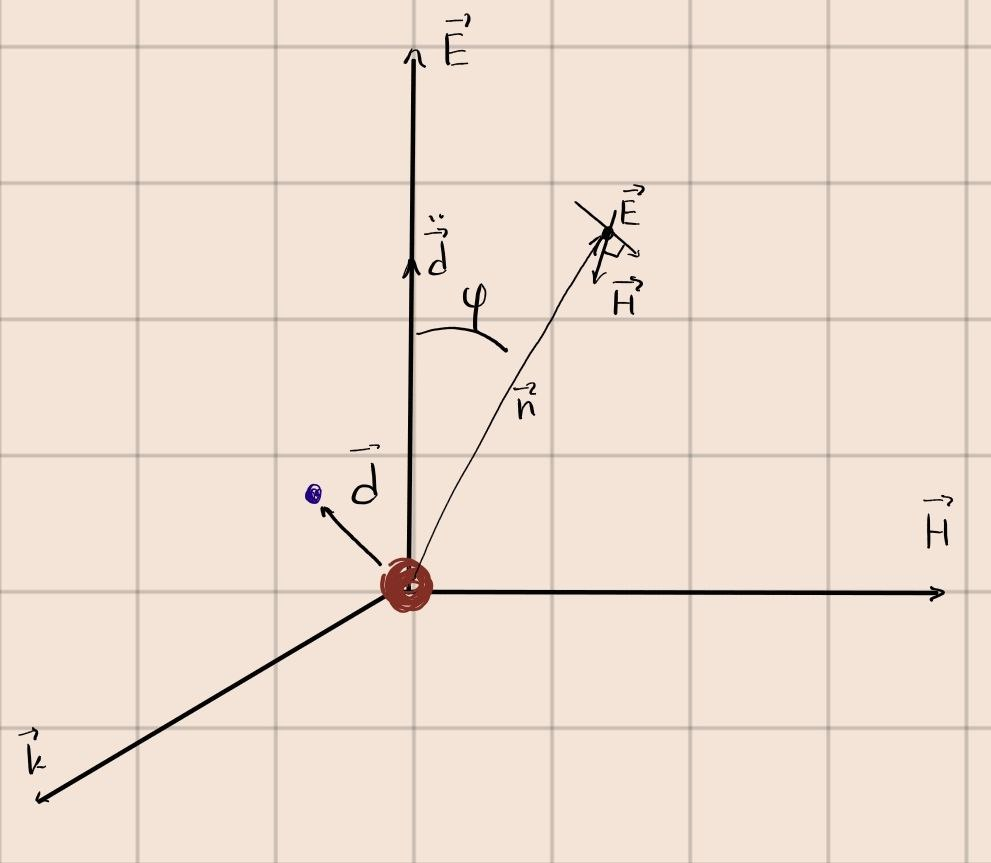
\includegraphics[trim={0 0 0 0},clip,width=\textwidth]{sours_img/sh.jpg}
    \label{pict}
\end{figure}

\subsection{Вектор пойнтинга}
Учитывая ортогональность векторов $H$ и $E$, также то что в 
монохроматической волне $\abs{H} = \abs{E}$, то вектор Пойнтинга
\begin{equation}
    S = \cfrac{cH^2}{4\pi}n.
\end{equation}
От сюда получим 
\begin{equation}
    d\mathfrak{I} = \cfrac{cH^2}{4\pi}R^2do
    \label{eq:2.7}
\end{equation}


\subsection{Частотное пространство}

Часто удобно работаь в спектральном разложении поэтому посмотрим 
на зависимомти в фурье образа. Напрямую из переобразования формул 
\ref{eq:2.5} получим:
\begin{gather}
    \begin{matrix}
        H_\omega = i \insqr{k, A_\omega},\\
        E_\omega = \cfrac{ic}{\omega} \insqr{k, \insqr{k, A_\omega}},
    \end{matrix}
\end{gather}
Воспользовавшись формулой 
\begin{equation}
    \int_\re f^2 dt = \int_\re \abs{f_\omega}^2 \cfrac{d\omega}{2\pi} 
    = 2\int_{\re_+} \abs{f_\omega}^2 \cfrac{d\omega}{2\pi} 
\end{equation}
Заметив что от в \ref{eq:2.7}  зависит от $t$ только посредстаом $H$ 
получим:
\begin{equation}
    d\mathfrak{I} = \cfrac{c}{2\pi} \abs{H}^2R^2do
    \label{eq:if}
\end{equation}
